 % use the "wcp" class option for workshop and conference
 % proceedings
 %\documentclass[gray]{jmlr} % test grayscale version
 %\documentclass[tablecaption=bottom]{jmlr}% journal article
 \documentclass[pmlr,twocolumn,10pt]{jmlr} % W&CP article
 
 \let\SUP\textsuperscript

% \usepackage{geometry}
% \geometry{margins=0.1in,textwidth=7in}

 % The following packages will be automatically loaded:
 % amsmath, amssymb, natbib, graphicx, url, algorithm2e

 %\usepackage{rotating}% for sideways figures and tables
 %\usepackage{longtable}% for long tables

 % The booktabs package is used by this sample document
 % (it provides \toprule, \midrule and \bottomrule).
 % Remove the next line if you don't require it.
\usepackage{tabto}    
\usepackage{graphicx}
\graphicspath{ {images/} }
\usepackage{float}
\usepackage{natbib}
\usepackage{url}

\usepackage{booktabs}
 % The siunitx package is used by this sample document
 % to align numbers in a column by their decimal point.
 % Remove the next line if you don't require it.
\usepackage[load-configurations=version-1]{siunitx} % newer version 
%\usepackage{siunitx}

 % The following command is just for this sample document:
\newcommand{\cs}[1]{\texttt{\char`\\#1}}% remove this in your real article

% The following is to recognise equal contribution for authorship
\newcommand{\equal}[1]{{\hypersetup{linkcolor=black}\thanks{#1}}}

% Customized Tabs
\newcommand\mytab{\hspace{10mm} \hspace{-5cm}}

 % Define an unnumbered theorem just for this sample document for
 % illustrative purposes:
\theorembodyfont{\upshape}
\theoremheaderfont{\scshape}
\theorempostheader{:}
\theoremsep{\newline}
\newtheorem*{note}{Note}

 % change the arguments, as appropriate, in the following:
\jmlrvolume{ML4H Extended Abstract Arxiv Index}
\jmlryear{2021}
\jmlrsubmitted{201}
\jmlrpublished{}
\jmlrworkshop{Machine Learning for Health (ML4H) 2021} % W&CP title

 % The optional argument of \title is used in the header
\title[NLP Techniques to Detect Cognitive Impairment]{Using Deep Learning to Identify Cognitive Impairment in Electronic Health Records}

 % Anything in the title that should appear in the main title but 
 % not in the article's header or the volume's table of
 % contents should be placed inside \titletag{}

 %\title{Title of the Article\titletag{\thanks{Some footnote}}}

\author{Tanish Tyagi \nametag{\thanks{Authors contributed equally}\SUP{1}},
Colin G. Magdamo\nametag{\footnotemark[1]\SUP{1}}, 
Ayush Noori \SUP{1},
Mayuresh Deodhar \SUP{1},
Zhuoqiao Hong \SUP{1},
Dimitry Propenko \SUP{1},
Rudy E. Tanzi \SUP{1},
Deborah Blacker \SUP{1},
Bradley T. Hyman \SUP{1},
Shibani S. Mukerji \SUP{1},
M. Brandon Westover \SUP{1},
Sudeshna Das\SUP{1},
\centering \Email{
\\[\bigskipamount] 
\SUP{1}\{ttyagi, 
cmagdamo,
anoori1,
...
sdas5\}
@mgh.harvard.edu}
% 
\begin{center}\addr Massachusetts General Hospital, Boston, MA\end{center}
}

\begin{document}

\maketitle

\begin{abstract}
\hspace{10mm} Dementia is a neurodegenerative disorder that causes cognitive decline and affects more than 50 million people worldwide. Dementia is under-diagnosed by healthcare professionals—only one in four people who suffer from dementia are diagnosed. Even when a diagnosis is made, it may not be entered as a structured diagnosis code in a patient’s charts.  Information relevant to cognitive impairment is often found within electronic health records (EHR) but manual review of clinician notes by experts is both time consuming and often prone to errors. Automated mining of these notes presents an opportunity to label patients with cognitive impairment (CI) in real-world data. In order to identify patients with cognitive impairment, we applied natural language processing (NLP) techniques. Model performance was compared to a baseline model that utilized structured features such as medication and ICD counts. % Add which model had highest performance %  
\end{abstract}

\begin{keywords}
EHR, NLP, Dementia
\end{keywords}

\section{Introduction}
\label{sec:intro} The possibility of early diagnosis of dementia is important for improving clinical outcomes and patient management of dementia. Often, a diagnosis is given once patient has reached moderate dementia, but irreversible damage has already been done to the brain. 
% https://www.dementiacarecentral.com/aboutdementia/facts/stages/ %
Yet, dementia is not formally diagnosed or coded in claims data for over 50\% of older adults living with probable dementia. Tools that can efficiently and effectively analyze medical records for warning signs of dementia and recommend patients for follow up with a specialist can be critical to obtaining early diagnosis for dementia. We aim to use NLP to detect signs of cognitive impairment from unstructured clinician notes by using deep learning techniques. An overview of our project can be found in Appendix A. 

\section{Related Works}
\label{sec:RelatedWorks} 

\section{Dataset, Preprocessing, and Annotations}
\label{sec:Dataset+Preprocessing+Annotations}

\paragraph{Dataset}
\label{sec:Dataset} Our gold-standard dataset consisted of a cohort (N = 16,428) of patients from the Mass General Brigham (MGB) HealthCare (formerly Partner's Healthcare, comprising two major academic hospitals, community hospitals, and community health centers in the Boston area) system who were older than 60 years (as of July 13, 2021) and had APOE genotype (biggest genetic risk factor for dementia) data available from the BioBank. Each patients' EHR record was then annotated by neurologists using a web-based annotation tool (UI Interface in Appendix A) as 1) Yes, i.e., patient has CI; 2) No i.e., Patient does not have CI; and 3) Neither i.e., sequence has no information on patient’s cognition. 
% link
\figureref{fig:fig1} shows examples of example sequences for all 3 classes. 

% Figure 1 - Example Sequences
\begin{figure*}[h!]
\label{fig:fig1}
\centering 
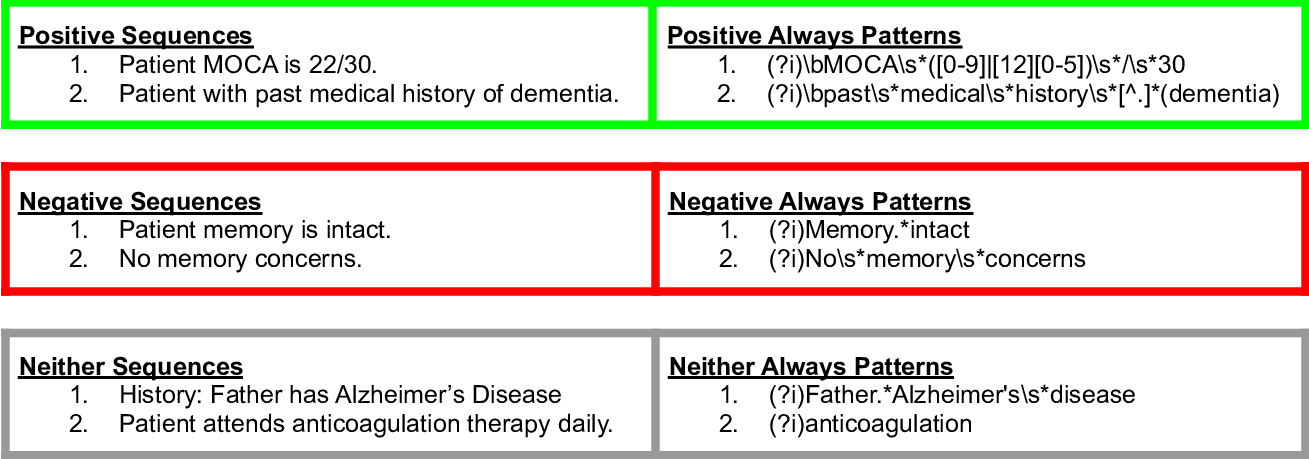
\includegraphics[scale = 0.35]{Figure-1.png}
\caption{Example Sequences}
\end{figure*}

\paragraph{Preprocessing}
\label{sec:Preprocessing} For each patient in our gold-standard dataset, we extracted unstructured clinician notes, identified matches to dementia-related keywords (Appendix B), and constructed sequences from the note text around each of these matches (of length 800 characters). Our cohort of 16,428 patients had 279,224 sequences in total. 

\paragraph{Annotations}
\label{sec:Annotations} We initially assigned 5,000 sequences diversified by keyword matches from 5,000 unique patients for neurologist labeling. In order to expedite annotations, we devised a scheme to known as "always patterns". An always pattern is defined as a phrase or regex expression that in any context indicates the phrase will be labeled with a particular class (i.e. yes, no, or neither). If an always pattern is inputted, all other sequences have language that matches with the phrase will be automatically labeled accordingly.

The final dataset was split between train (95\%) and holdout test (5\%) sets, stratified across label and proportion of sequences annotated manually and through always patterns. % {Will change} % 
Validation datasets were split from the train set using techniques described in the Methodology section. \tableref{tab:table1} shows demographics of the cohort of patients.  

%% Table 1 - Demographics of Dataset %%
\begin{table*}[hbtp]
\floatconts
{tab:table1}
\centering 
    {
        \begin{tabular}{lccc}
        \toprule
        \bfseries Characteristic & \bfseries (N = 16428) \\
        \midrule
        \textbf{Age (years) mean (SD)} & \fseries 73.01 (7.96) \\ 
        \textbf{Gender Male, \emph n (\%)}  & \fseries 8740 (53.2)\\ 
        \textbf{Race, \emph n (\%)} \\ 
            \hspace{10mm} White & 14896 (90.7) \\
            \hspace{10mm} Other/Not Recorded & 608 (3.7) \\
            \hspace{10mm} Black & 570 (3.5) \\
            \hspace{10mm} Hispanic & 170 (1.0) \\
            \hspace{10mm} Asian & 168 (1.0) \\
            \hspace{10mm} Indigenous & 16 (0.01) \\
        \textbf{APOE Genotype, \emph n (\%)} \\ 
            \hspace{10mm} {APOE ${\bm{\varepsilon}}$2 & 2028 (12.3)} \\
            \hspace{10mm} {APOE ${\bm{\varepsilon}}$3 & 10177 (62.0)} \\
            \hspace{10mm} {APOE ${\bm{\varepsilon}}$4 & 4223 (25.7)} \\
        \textbf{Average Speciality Visits (SD)} & 1.67 (4.6) \\ 
        \textbf{Average PCP Encounters (SD)} &  5.25 (5.63) \\ 
        % \textbf{Encounters AVG (SD)} & 14.55 (23.2) \\
        % \textbf{Keyword Matches AVG (SD)} & 26 (54.03) \\
        \bottomrule
        \end{tabular}
        {\caption{Demographics of Data}} \\
    }
\end{table*}

\section{Methodology}
\label{sec:Methodology}  
% {We built 4 models and compared performance to the baseline model. It is important to note that these models were trained on binary labels, despite annotators labeling sequences with 3 classes. This was done because our overall task was to classify if a patient had CI, not whether a sequence indicates CI. % phrase better % 
% A label of neither does not pertain  patient can only be classified as having or not having CI. In order to convert this problem to binary labels, we aggregated no and neither labels to class 0 and yes labels to class 1. }

% \label{sec:Baseline}  
% \paragraph{(1) Baseline Model} We performed L1 regularized logistic regression where the cognitive concern label was regressed on the counts of medications, keyword counts, and ICD codes relevant to CI. The lambda value was selected through 10-fold Cross Validation (CV) to maximize the average area under the Receiver Operator Characteristic (ROC). % {To be implemented} %

\label{sec:TFIDF}  
\paragraph{(1) Logistic Regression with TF-IDF Vectors} We performed TF-IDF (term frequency-inverse document frequency) vectorization on the annotated sequences and selected features based on a term's Pearson correlation coefficient with the outcome. L1 Regularized logistic regression was applied with the annotated cognitive impairment labels. We used different correlation coefficients as thresholds to select features and iterated over different lambda values to determine the optimal lambda value and correlation coefficient threshold. 

% \label{sec:Baseline+TFIDF}  
% \paragraph{(3) Model 1 + Model 2} % {TBD} % 

\label{sec:Transformer}  
\paragraph{(2) Transformer Based Sequence Classification Language Model} We utilized a pre-trained language model called Clinical-BERT, which was trained on the MIMIC II database containing EHR records from ICU patients. We used the implementation in the Huggingface Transformer and Simpletransformers packages. After text preprocessing, input texts were tokenized with the default tokenizer and converted to embeddings. The model was initialized with pre-trained parameters and later fine-tuned on our labeled training set. Optuna was used to perform a 20-trial study and tune the learning rate, adam epilson, and the number of train epochs on the held-out validation set. 

\section{Results}
\label{sec:Results}  
% talk abt performance
% which patients are correctly classified for each model
% compare conf mat's for each model
% distribution of CI/not CI labels
% talk about different patient aggregation scheme
% address lack of not patient level labels
% TFIDF might have lot of false positives b/c of use of vocab that doesn't discuss patient, deep learning will be able to use context
% start with justification to aggregation to patient level
% sensivity should hopefully improve, deep learning should reduce specificity b/c of use of contextual information
% discuss if certain patients were predicted differently for all models
% some ppl will be classified as 0, until deep learning, where it will be hopefully changed to 1
% group of ppl who get 0 for baseline, prediction of 1 with tf-idf and deep
% group of ppl who get 1 for tf-idf, 0 for deep learning b/c of high false positive rate, vocab cld be talking abt family member (tf-idf will address underdiagnosis, deep learning will address misdiagnosis better) 
% tf-idf is easy to "trigger", deep learning will evaulate based on context
% Talk about Stats
% TF-IDF model struggles with understanding context of words around keyword match
% Future plans include reducing false positives by gathering more annotated sequences and using deep learning natural language. Currently, many of our false positives are from the model identifying the presence of a keyword but struggling to understand the context around the keyword match; many of these contexts negate the presence of CI for the patient in question. Deep Learning can leverage contextual information, making it promising for this task.

We evaluated each model using a prediction threshold to maximize the accuracy and calculated performance metrics based on that threshold. Model performance for each model in shown in \tableref{tab:table2}. All performance metrics are based on the sequence level class assignments. % discuss sequence level stats (notes above)% 

In order to obtain a patient level class assignment assignments from the models,  %discuss%

% Table 2 - Results
\begin{table*}[hbtp]
\floatconts
{tab:table2}
  {\begin{tabular}{lcccccccc}
    \toprule 
    % add precision and recall, 
    \bfseries Model & \bfseries AUC & \bfseries Accuracy & \bfseries Sensitivity & \bfseries Specificity & \bfseries Micro F1  & \bfseries Macro F1 & \bfseries Weighted F1 \\ 
    \midrule
    TF-IDF & 0.95 & 0.84 & 0.83 & 0.92 & 0.84 & 0.81 & 0.84 \\
    ClincialBERT & 0.98 & 0.93 & 0.91 & 0.96 & 0.93 & 0.92 & 0.93 \\
    \bottomrule
  \end{tabular}}
  {\caption{Model Performance}}
\end{table*}

% \begin{figure*}[h!]
% \label{fig:fig2}
% \centering 
% \includegraphics[scale = 0.75]{tfidf_patient_predictions.png}
% \caption{Patient Predictions for TF-IDF}
% \end{figure*}

% Table 3 + 4 - Relation of Med/ICD Codes to Model Predictions
% \begin{table*}[hbtp]
% \floatconts
% {tab:table3}
% \centering 
%   {\begin{tabular}{cccccc}
%     \toprule 
%     \bfseries  & \bfseries Count & \bfseries Yes (\%) & \bfseries No/Ntr (\%)  & \bfseries Med/ICD Code (\%)  \\ 
%     \midrule
%     \bfseries{APOE ${\bm{\varepsilon}}$2} & \fseries 1754 & \fseries 0.15 & \fseries 0.85 & \fseries 0.11  \\
%     \bfseries{APOE ${\bm{\varepsilon}}$3} & \fseries 8751 & \fseries 0.15 & \fseries 0.85 & \fseries 0.11  \\
%     \bfseries{APOE ${\bm{\varepsilon}}$4} & \fseries 3436 & \fseries 0.18 & \fseries 0.82 & \fseries 0.17  \\
    
%     \bottomrule
%   \end{tabular}}
% {\caption{Comparison between Other Indicators of Cognitive Impairment and TF-IDF}} \\
% \end{table*}

\begin{table*}[hbtp]
\floatconts
{tab:table4}
\centering 
    {\begin{tabular}{cccccc}
    \toprule 
    \bfseries  & \bfseries Count & \bfseries Yes (\%) & \bfseries No/Ntr (\%)  & \bfseries Med/ICD Code (\%) \\ 
    \midrule
    \bfseries{APOE ${\bm{\varepsilon}}$2} & \fseries 1754 & \fseries 0.17 & \fseries 0.83 & \fseries 0.11  \\
    \bfseries{APOE ${\bm{\varepsilon}}$3} & \fseries 8751 & \fseries 0.17 & \fseries 0.83 & \fseries 0.11  \\
    \bfseries{APOE ${\bm{\varepsilon}}$4} & \fseries 3436 & \fseries 0.21 & \fseries 0.79 & \fseries 0.17  \\
    
    \bottomrule
  \end{tabular}}
  {\caption{Comparison between Other Indicators of Cognitive Impairment and Clinical-BERT}} \\
\end{table*}

\begin{figure*}[h!]
\label{fig:fig2}
\centering 
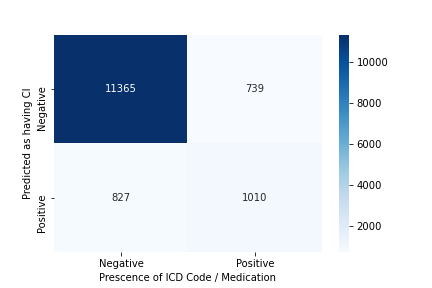
\includegraphics[scale = 0.75]{bert_patient_predictions.png}
\caption{Patient Level Predictions for ClinicalBERT}
\end{figure*}

%% Conclusion + Future Work %%
\section{Conclusion and Future Work} 
\label{sec:ConclusionFutureWork} We applied innovative Machine Learning and Deep Learning NLP techniques to identify patients with cognitive impairment in EHR. Our work can help combat the issues of underdiagnosis and misdiagnosis for dementia. % {More coming soon } %

\clearpage
\appendix

% Appendix A
% Figure 2 - Overview
\section{Overview}
\label{fig:fig2}
\begin{figure}[h]
\centering 
\includegraphics[scale = 0.14]{Overview.png}
\caption{Overview}
\end{figure}

\clearpage

% Appendix B
\section{Keywords} 
\begin{table}[hbtp] 
\floatconts
{app:keywords}
    {\begin{tabular}{lccc}
        \toprule
        \bfseries Keyword & \bfseries Match Count\\
        \midrule
        
        \textbf{Memory} & \fseries 109218 \\ 
        \textbf{Cognition}  & \fseries 87655 \\ 
        \textbf{Dementia} & \fseries 51034 \\ 
        \textbf{Cerebral} & \fseries 45886 \\ 
        \textbf{Cerebrovascular} & \fseries 36370 \\ 
        \textbf{Cerebellar} & \fseries 26863 \\
        \textbf{Cognitive Impairment} & \fseries 20267 \\ 
        \textbf{Alzheimer} & \fseries 20581 \\ 
        \textbf{MOCA} & \fseries 9767 \\ 
        \textbf{Neurocognitive} & \fseries 7711 \\ 
        \textbf{MCI} & \fseries 3889 \\ 
        \textbf{Amnesia} & \fseries 3695 \\ 
        \textbf{AD} & \fseries 2673 \\ 
        \textbf{Lewy} & \fseries 2561 \\ 
        \textbf{MMSE} & \fseries 2134 \\ 
        \textbf{LBD} & \fseries 224 \\ 
        \textbf{Corticobasal} & \fseries 147 \\ 
        \textbf{Pick's} & \fseries 41 \\ 
        
        \bottomrule
        \end{tabular}}
        {\caption{Keywords indicative of Cognitive Impairment}} \\

\end{table}
% \clearpage

% Appendix C
\section{Top TF-IDF Word Features}
\begin{table}[hbtp]
    {\begin{tabular}{cccc}
    \toprule 
    \bfseries Word & \bfseries Corr & \bfseries Word & \bfseries Corr &
    \midrule
    
    \textbf{Intact} & \fseries 0.56 & \textbf{Experiences} & \fseries 0.36 \\
    \textbf{Oriented} & \fseries 0.43 & \textbf{Associations} & \fseries 0.36 \\ 
    \textbf{Concentration} & \fseries 0.42 & \textbf{Homicidal} & \fseries 0.36 \\ 
    \textbf{Orientation} & \fseries 0.41 & \textbf{Observation} & \fseries 0.36 \\
    \textbf{Sensorium} & \fseries 0.40 & \textbf{Knowledge} & \fseries 0.36 \\ 
    \textbf{Perceptions} & \fseries 0.40 & \textbf{Abstract} & \fseries 0.36 \\
    \textbf{Judgement} & \fseries 0.39 & \textbf{Suicidal} & \fseries 0.35 \\
    \textbf{Fund} & \fseries 0.38 & \textbf{Attention} & \fseries 0.35 \\
    \textbf{Insight } & \fseries 0.36 & \textbf{Content} & \fseries 0.34 \\ 
    \textbf{Ideation} & \fseries 0.36 & \textbf{Thought} & \fseries 0.34  \\  
    
    \bottomrule
  \end{tabular}}
\end{table}
\clearpage


\end{document}
